\subsection{Workflow dentro do Flux que utiliza das funções}

\subsubsection{Workflows BPL}

Os workflows laboratoriais de nome BPL (Boas Práticas de Laboratório) estavam separados em 5 workflows diferentes, já que existiam BPMs diferentes para cada tipo de usuário.
O problema com o BPL é que existem workflows pequenos (pouco profundos, com poucas atividades) e também existem workflows grandes (Com muitas atividades, profundos) e, com isso, surge a dificuldade de disponibilização de dados para diferentes tipos de usuários como a utilização do workflow por gerentes e técnicos de laboratório.

Essa dificuldade existe porque, para cada workflow, deve ser acessado uma página diferentes do LIMS, já que cada um desses workflows representa um sistema diferente para cada usuário.

Com a implementação de workflows dinâmicos, é possível acessar as informações de atividades profundas de maneira pontual, a depender das necessidades do usuário, que pode escolher em qual atividade ele quer centralizar a visualização para continuar seus trabalhos.

Caso um gerente queira ver resultados de algum experimento feito por seu funcionário, ele também pode acessar o mesmo workflow e centralizar em uma atividade diferente da que foi centralizada pelo técnico de laboratório, fazendo com que a interface seja dinâmica para cada usuário e os trabalhos sejam mais focados na inserção e coleta de dados no sistema e não na procura dos mesmos.

Para que esta ferramenta fosse mais poderosa, também foi implementado a funcionalidade de múltiplas atividades iniciais no workflow do BPL, fazendo com que workflows dinâmicos pudessem ser centralizados em qualquer atividade que estivesse compartilhada entre instâncias, agregando informações necessárias para execução de um BPM, como calibração de um equipamento de análise de substâncias.

Com isso, 5 workflows foram agregados, transformando-os em um grande BPM com 5 atividades iniciais. As atividades que foram compartilhadas foram \textbf{Atividades compartilhadas}, dando a possibilidade de cientistas que fazem as análises de substâncias trocarem informações com técnicos de laboratório que fazem a calibração de máquinas para informar que uma máquina necessita de calibração ou o caminho contrário, técnicos de laboratório disponibilizarem a informação que a calibração de uma máquina está pronta.

\subsubsection{CTTX e BPL-Equipamentos}

O workflow mencionado anteriormente, compartilhando a atividade de calibração entre os workflows CTTX e BPL - Equipamentos foi implementado no Flux para uso laboratorial, adaptando os dois workflows para que houvesse a comunicação entre as equipes que trabalham no laboratório.

A estrutura dentro do Flux fica demonstrada pela figura~\ref{fig:cttx_bpl_flux}, que pode ser acessada dentro do próprio software. Na figura, podemos ver referência à atividade ``Calibração" nos dois fluxos de trabalho. Para separar quais atividades ficam disponíveis para cada usuário do sistema, é necessário utilizar o sistema de permissões já implementado no Flux para especificar permissões de visualização, execução e aprovação da atividade.

\begin{figure}
    \centering
    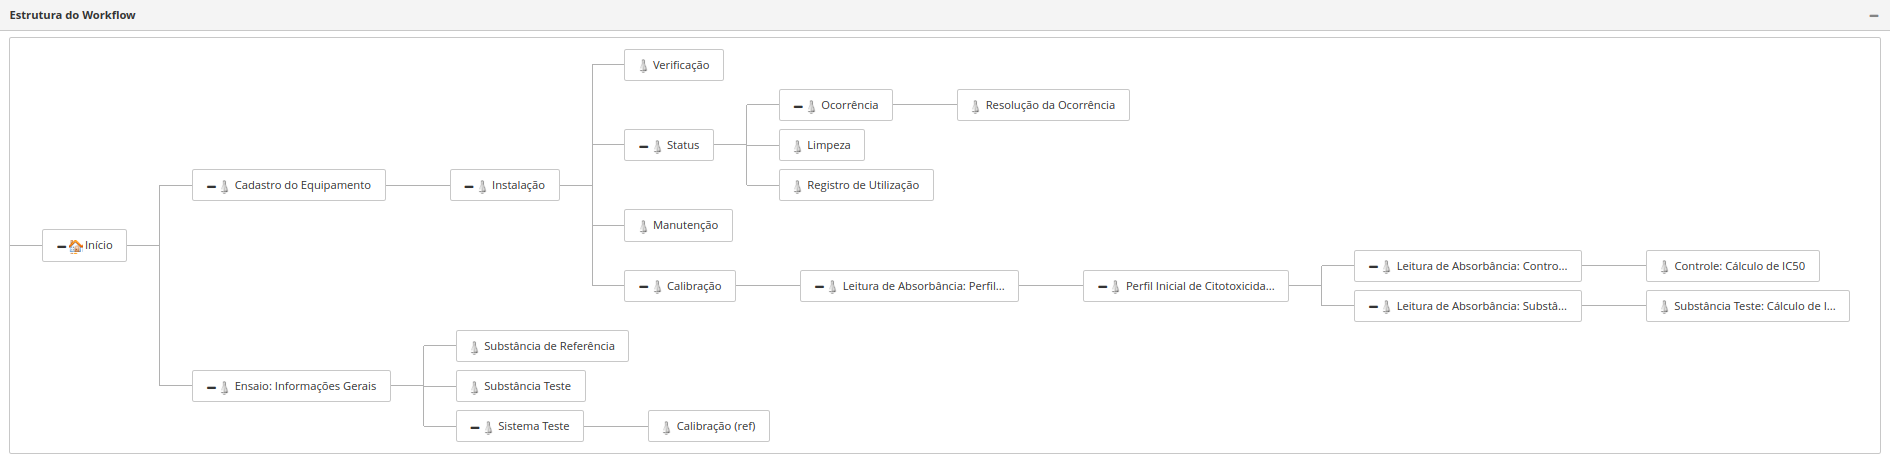
\includegraphics[width=1\textwidth]{imgs/CTTX-EQP/estrutura_cttx_eqp_flux.png}
    \caption{Estrutura do workflow conjunto CTTX com BPL - Equipamentos demonstrada pela interface do Flux. Como podemos ver pela imagem, após a atividade ``Sistema teste" (canto inferior da imagem), temos a atividade ``Calibração (ref)", que refere-se a atividade calibração no fluxo de trabalho demonstrado logo acima.}
    \label{fig:cttx_bpl_flux}
\end{figure}

Assim, podem ser separados usuários que irão executar a atividade de calibração do equipamento de usuários que irão realizar os experimentos a partir daquela calibração, diminuindo os erros que podem ocorrer caso as atividades sejam disponibilizadas sem que um equipamento tenha sido calibrado corretamente.

